\documentclass[12pt, a4paper]{report}
\usepackage{caption, subcaption}
\usepackage[utf8]{inputenc}
\usepackage[italian]{babel}
\usepackage[T1]{fontenc}
\pdfminorversion=4
\usepackage{graphicx}
\usepackage{geometry}
\geometry{ left=3cm, right=3cm, top=3cm, bottom=3cm }
\usepackage{tabularx}
\usepackage{titlesec}
\usepackage{etoolbox}
\usepackage{colortbl}
\usepackage{csquotes}
\usepackage{graphicx}
\usepackage{textcomp}
\usepackage{titling}
\usepackage{amsmath}
\usepackage{amssymb}
\usepackage{xcolor}
\usepackage{array}
\usepackage{float}


\newcolumntype{C}[1]{>{\centering\arraybackslash}p{#1}}
\renewcommand{\chaptername}{Capitolo}

\title{Laboratorio di Fisica dei Plasmi}
\author{Negrini Filippo}
\date{A.A. 2023/2024}


\begin{document}

\begin{titlepage}
    \centering
    \vspace*{2cm}
    {\Huge \thetitle\par}
    \vspace{1cm}
    {\Large \theauthor\par}
    \vspace{0.2cm}
    {\Large \thedate\par}

    \vfill
    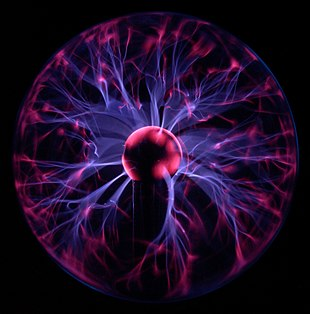
\includegraphics[width=0.8\textwidth]{Immagini/PlasmaLamp.jpg}
    \vfill
\end{titlepage}
\newpage
\tableofcontents
\newpage
\chapter{Introduzione}

Nel corso di Laboratorio di Fisica dei Plasmi siamo interessati a plasmi non neutri, ossia dei sistemi a molti corpi
costituiti da particelle cariche, che presentano una carica netta globale. Sistemi di questo genere sono caratterizzati
dalla presenza di forti campi elettrici legati alla natura non neutra dell'insieme di particelle considerato: tali campi
possono avere grande influenza sul comportamento del plasma e sulle proprietà del regime di stabilità che si può instaurare.
I plasmi generati in laboratorio sono plasmi di elettroni: essi vengono confinati utilizzando una trappola di Malmberg-Penning.

\section{Struttura della dispensa}

La dispensa si articola nei seguenti capitoli:
\begin{enumerate}
    \item In questo capitolo abbiamo introdotto la tipologia di fenomeni fisici che ci proponiamo di trattare
    e studiare sperimentalmente.
    \item Nel Capitolo 2 vengono introdotte alcune tecniche teoriche che consentono di studiare le caratteristiche principali
    dei plasmi non-neutri, ponendo particolare enfasi sugli equilibri che interessano le esperienze di laboratorio.
  \end{enumerate}

\newpage
\chapter{Modelli teorici}

In questo capitolo investighiamo gli approcci teorici che consentono di trattare un plasma non collisionale e non neutro: ciò
vuol dire che il sistema presenta una carica netta e che le proprietà sono studiate per intervalli di tempo piccoli rispetto
alle tempistiche medie fra collisioni. Per descrivere un tale plasma possonon essere utilizzati due formalismi:
\begin{itemize}
    \item \textit{trattazione di fluido macroscopico}, basata sulle equazioni di Maxwell e sull'equazione dei momenti
    \item \textit{trattazione cinetica}, basata sulle equazioni di Vlasov-Maxwell
\end{itemize}
Nella prima delle due descrizioni vengono presi in considerazione osservabili macroscopici quali $n\left(\vec{x},\,t\right)$, 
$V\left(\vec{x},\,t\right)$ e $P\left(\vec{x},\,t\right)$: tali quantità evolvono in dipendenza dei campi elettrici e magnetici
presenti, che possono essere determinati mediante le equazioni di Maxwell. Se il plasma in analisi è freddo è possibile trascurare
le variazioni di pressione, ponendo a zero la varianza del tendore delle pressioni. Il vantaggio di un tale approccio è la sua 
elevata semplicità: in ambito fluido non è però possibile trattare instabilità collettive e fenomeni caratteristici di un plasma, 
come il Landau damping.

Per includere la fenomenologia termica nell'analisi del plasma è necessario utilizzare un approccio \textit{cinetico}: in questo
caso l'attenzione è rivolta alla distribuzione $f\left(\vec{x},\,\vec{p},\,t\right)$, che descrive la densità di probabilità di 
avere il sistema nel punto $\left(\vec{x},\,\vec{p}\right)$ dello spazio delle fasi al tempo $t$. Per come è definita la
distribuzione $f$, abbiamo che
$$f\left(\vec{x},\,\vec{p},\,t\right)d^3xd^3p\,=\,\text{numero medio di particelle nell'intorno di } \left(\vec{x},\,\vec{p}\right)$$
Questo approccio consente di studiare un'ampia classe di fenomeni collettivi che dipendono dalla struttura della distribuzione
all'equilibrio nello spazio delle fasi.

\section{Trattazione cinetica}

Consideriamo un plasma non neutro di elettroni caratterizzati da carica $e$ e massa $m$: per scale di tempo corte rispetto
al tempo di collisione la funzione di distribuzione di singola particella $f\left(\vec{x},\,\vec{p},\,t\right)$ evolve secondo
l'equazione di Vlasov, che descrive l'evoluzione incomprimibile secondo il teorema di Liouville nello spazio delle fasi
6-dimensionale $\left(\vec{x},\,\vec{p}\right)$.
\begin{equation}
    \left\{\frac{\partial}{\partial t}\,+\,\vec{v}\cdot\frac{\partial}{\partial \vec{x}}\,+\,e\left(\vec{E}\,+\,\frac{\vec{v}\times\vec{B}}{c}\right)\cdot\frac{\partial}{\partial \vec{p}}\right\}f\left(\vec{x},\,\vec{p},\,t\right)\,=\,0
    \label{equation: VlasovEq}
\end{equation}
Notiamo che è presente un termine in cui figurano sia il campo elettrico che il campo magnetico: possiamo determinarli utilizzando le
equazioni di Maxwell
\begin{align}
    &\nabla \times \vec{E} = -\frac{1}{c}\left[c\right]\frac{\partial \vec{B}}{\partial t} \\
    &\nabla \times \vec{B} = \frac{4\pi}{c}\left[\frac{\mu_0 c}{4\pi}\right]e\int{d^3p\vec{v}f(\vec{x},\,\vec{p},\,t)} + \frac{4\pi}{c}\left[\frac{\mu_0 c}{4\pi}\right]\vec{J}_{ext} + \frac{1}{c}\left[\frac{1}{c}\right] + \frac{\partial \vec{E}}{\partial t} \\
    &\nabla \cdot \vec{E} = 4\pi\left[\frac{1}{4\pi\varepsilon_0}\right]e\int{d^3p f\left(\vec{x},\,\vec{p},\,t\right)} + 4\pi\left[\frac{1}{4\pi\varepsilon_0}\right]\rho_{ext} \\
    &\nabla \cdot \vec{B} = 0
\end{align}
Le equazioni di Vlasov-Maxwell sono altamente non lineari, in quanto $f\left(\vec{x},\,\vec{p},\,t\right)$ è modificata dai campi auto-indotti
dal plasma, che a loro volta evolvono quando la funzione di distribuzione cambia. In condizioni di stato quasi-stazionario è possibile
porre a zero tutte le derivate parziali rispetto al tempo in modo da determinare le soluzioni stazionarie $f^0\left(\vec{x},\,\vec{p}\right)$,
$\vec{E}^0\left(\vec{x}\right)$ e $\vec{B}^0\left(\vec{x}\right)$: lavorando con piccole perturbazioni è possibile valutare la stabilità
degli equilibri così individuati.

\section{Trattazione fluida}

In alcune circostanze il comportamento globale del plasma può essere descritto utilizzando un'approccio fluido-dinamico: 
siamo interessati alla densità del sistema $n\left(\vec{x},\,t\right)$, alla velocità media $\vec{V}\left(\vec{x},\,t\right)$,
al momento medio $\vec{P}\left(\vec{x},\,t\right)$ ed al tensore delle pressioni $\mathbf{P}\left(\vec{x},\,t\right)$. Per 
passare dalla trattazione cinetica a quella fluida introduciamo i primi momenti della distribuzione $f\left(\vec{x},\,\vec{p},\,t\right)$ 
integrando nei momenti, in modo tale da perdere l'informazione cinetica e mantenere solo quella spaziale. Possiamo quindi 
riconoscere:
\begin{equation}
    n\left(\vec{x},\,t\right)\,=\,\int d^3p \,f\left(\vec{x},\,\vec{p},\,t\right)
    \label{equation: numb_density}
\end{equation}
\begin{equation}
    n\left(\vec{x},\,t\right)\vec{V}\left(\vec{x},\,t\right)\,=\,\int d^3p\,\vec{v} f\left(\vec{x},\,\vec{p},\,t\right)
    \label{equation: mean_velocity}
\end{equation}
\begin{equation}
    n\left(\vec{x},\,t\right)\vec{P}\left(\vec{x},\,t\right)\,=\,\int d^3p\,\vec{p} f\left(\vec{x},\,\vec{p},\,t\right)
    \label{equation: p_tens}
\end{equation}
\begin{equation}
    \mathbf{P}\left(\vec{x},\,t\right)\,=\,\int d^3p\left[\vec{p}\,-\,\vec{P}\left(\vec{x},\,t\right)\right]\left[\vec{v}\,-\,\vec{V}\left(\vec{x},\,t\right)\right] f\left(\vec{x},\,\vec{p},\,t\right)
    \label{equation: p_tens1}
\end{equation}
Possiamo ora ottenere le equazioni fluide andando ad integrare nei momenti: la semplice integrazione in $d^3p$ restituisce 
l'equazione di continuità, mentre lavorando con $\vec{p}d^3p$ è possibile ottenere l'equazione che descrive l'equilibrio delle
forze:
\begin{equation}
    \frac{\partial n}{\partial t}\,+\,\nabla \cdot \left(n\vec{V}\right)\,=\,0
    \label{equation: continuity_eq}
\end{equation}
\begin{equation}
    n\left(\frac{\partial}{\partial t}\,+\,\vec{V}\cdot \nabla\right)\vec{P}\,+\,\nabla \cdot \mathbf{P}\,=\,nq\left(\vec{E}\,+\,\frac{1}{c}\left[c\right]\vec{v} \times \vec{b}\right)
    \label{equation: force_balance}
\end{equation}
Abbiamo trovato un sistema di equazioni differenziali in cui nell'equazione che descrive l'evoluzione del momento di ordine 0 
compare il momento di primo ordine ed in generale nell'equazione riguardante il k-esimo momento è presente il k+1-esimo: per 
chiudere il sistema supponiamo di trattare un plasma freddo, ossia caratterizzato da velocità termica molto inferiore alla 
velocità fluida in gioco. Così facendo possiamo trascurare il termine di ordine superiore, ossia la divergenza del tensore delle 
pressioni, di fatto trascurando l'agitazione termica rispetto ai moti del fluido.

\section{Equilibrio di rotazione}

Consideriamo un plasma non-neutro di lunghezza infinita confinato radialmente da un campo magnetico $\vec{B}\,=\,B_0 \hat{e}_z$: 
in condizioni di stato stazionario $\left(\partial/\partial t\,=\,0\right)$ supponiamo di avere un profilo di densità a gradino 
assi-simmetrico del tipo:
\begin{equation}
    n\left(r\right)\,=\,
\begin{cases}
    n_0 \qquad \qquad r \in \left[0,\,r_b\right] \\
    0\,\,\, \qquad \qquad r \in \left(r_b,\,\infty\right)
\end{cases}
\label{equation: eq_density}
\end{equation}
\begin{figure}[H]
    \centering
    \includegraphics[width=0.9\textwidth]{Immagini/ProfiliDensità.png}
    \caption{Confronto fra profilo di densità ideale e situazione realistica}
    \label{figure: ProfDens}
\end{figure}
La distribuzione spaziale di carica genera un campo elettrico diretto radialmente ed identicamente nullo nel centro del 
plasma: è possibile determinare l'andamento di tale campo risolvendo l'equazione di Poisson. Il set di equazioni che consente 
di descrivere la situazione in analisi è:
\begin{equation}
    \nabla \cdot \left(n\vec{V}\right)\,=\,0
    \label{equation: conteq_steadystate}
\end{equation}
\begin{equation}
    \left(\vec{V}\cdot \nabla\right)\vec{V}\,=\,\frac{q}{m}\left(-\nabla\Phi\,+\,\frac{1}{c}\left[c\right]\vec{v} \times \vec{b}\right)
    \label{equation: forcebalance_steadystate}
\end{equation}
\begin{equation}
    \nabla^2\Phi\,=\,-4\pi\left[\frac{1}{4\pi\varepsilon_0}\right]qn
    \label{equation: Poisson_steadystate}
\end{equation}
Procediamo con l'obiettivo di determinare il potenziale: sfruttiamo le simmetrie del sistema, evidenti nel set di coordinate
cilindriche $\left(r,\,\theta,\,z\right)$. Dato che non abbiamo dipendenza dalla coordinata $z$, tutte le derivate rispetto alla 
quota saranno identicamente nulle. L'equazione di continuità e l'equazione di evoluzione dei momenti si traducono in:
\begin{align}   % FARE UN CHECK: INDICI POTREBBERO ESSERE ERRATI
    & \frac{1}{r}\frac{\partial}{\partial r}\left(rnV_z\right)\,+\,\frac{1}{r}\frac{\partial}{\partial \theta}\left(nV_\theta\right)\,=\,0 \\
    & V_r\frac{\partial V_z}{\partial r}\,+\,\frac{V_\theta}{r}\frac{\partial V_z}{\partial V_\theta}\,-\,\frac{V^2_\theta}{r}\,=\,\frac{q}{m}\left(-\frac{\partial \Phi}{\partial r}\,+\,\frac{1}{c}\left[c\right]V_\theta B_\theta\right) \\
    & V_r\frac{\partial V_\theta}{\partial r}\,+\,\frac{V_\theta}{r}\frac{\partial V_\theta}{\partial \theta}\,+\,\frac{V_\theta V_r}{r}\,=\,-\frac{q}{m}\left(\frac{1}{r}\frac{\partial \Phi}{\partial \theta}\,+\,\frac{1}{c}\left[c\right]V_zB_\theta\right) \\
    & \frac{1}{r}\frac{\partial}{\partial r}\left(r\frac{\partial \Phi}{\partial r}\right)\,+\,\frac{1}{r^2}\frac{\partial^2\Phi}{\partial \theta ^2}\,=\,-4\pi\left[\frac{1}{4\pi\varepsilon_0}\right]qn
\end{align}
Specializzando la casistica in analisi sfruttando il profilo di densità introdotto in precedenza \eqref{equation: eq_density} ed imponendo 
delle ulteriori condizioni di simmetria sulla velocità:
\begin{equation}
\begin{cases}
    n\,=\,n\left(r\right) \\
    V_r\,=\,0   \\
    V_\theta\,=\,V_\theta\left(r\right)
\end{cases}
\end{equation}
è possibile ridurre il set di partenza a sole due equazioni che consentono di ottenere infomazioni riguardo al comportamento 
globale del plasma. 
\begin{figure}[H]
    \centering
    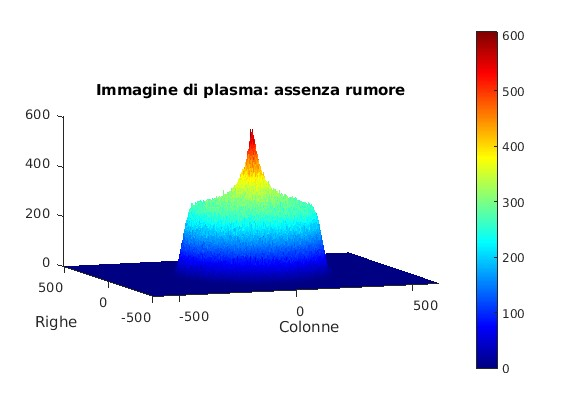
\includegraphics[width=0.9\textwidth]{Immagini/RealPlasma.jpg}
    \caption{Immagine di plasma scattata in laboratorio dove notiamo come il profilo di densità risulti alquanto lontano dalle
    condizioni di idealità. }
    \label{figure: RealPlasma}
\end{figure}
Noto il profilo di densità, risolviamo inizialemente il problema di Poisson per poi ottenere delle informationi 
sulla velocità azimutale, che sarà quella caratteristica di un moto di rotazione rigida. Procediamo con l'analisi delle equazioni 
ridotte per merito delle assunzioni precedentemente giustificate:
\begin{equation}
    -\frac{V_\theta^2}{r}\,=\,\frac{q}{m}\left(-\frac{\partial \Phi}{\partial r}\,+\,\frac{1}{c}\left[c\right]V_\theta B_\theta\right)
    \label{equation: reduced_Poisson}
\end{equation}
\begin{equation}
    \frac{1}{r}\frac{\partial}{\partial r}\left(r\frac{\partial \Phi}{\partial r}\right)\,=\,-4\pi\left[\frac{1}{4\pi\varepsilon_0}\right]qn
    \label{equation: reduced_momentum}
\end{equation}
L'equazione \eqref{equation: reduced_momentum} deve essere risolta separatamente nelle due regioni in cui può essere diviso lo spazio 
utilizzando come criterio la densità di carica:
\begin{equation}
    \frac{1}{r}\frac{\partial}{\partial r}\left(r\frac{\partial \Phi}{\partial r}\right)\,=\,
    \begin{cases}
        \alpha n_0 \,\,\,\, \qquad \qquad r \in \left[0,\,r_p\right] \\
        0 \qquad \qquad \qquad r \in \left[r_p,\,r_W\right]
    \end{cases}
    \label{equation: Poisson_step1}
\end{equation}
dove la costante alfa è definita come
\begin{equation}
    \alpha\,=\,4\pi e\left[\frac{1}{4\pi\varepsilon_0}\right]
\end{equation}
Per avere un problema ben definito è necessario imporre delle condizioni al contorno di senso fisico: vogliamo evitare una 
soluzioni divergente richiedendo che
\begin{equation}
    \begin{cases}
    \Phi \left(r\,=\,r_W\right)\,=\,0, \\
    \Phi \left(r\,=\,0\right)\,<\,\infty.
    \end{cases}
    \label{equation: BC}
\end{equation}
Integrando il problema di Poisson in entrambe le regioni prese in considerazione ed imponendo continuità e derivabilità in 
$r\,=\,r_p$ per giuntare le soluzioni si ottiene che
\begin{equation}
    \Phi\left(r\right)\,=\,\frac{m}{e}\omega_p^2
    \begin{cases}
        \frac{r^2\,-\,r_p^2}{4}\,+\,\frac{r_p^2}{2}\log{\left(\frac{r_p}{r_w}\right)}   \\
        \frac{r_p^2}{2}\log{\left(\frac{r}{r_W}\right)}
    \end{cases}
    \label{equation: potential_solution}
\end{equation}
dove si indica con $\omega_p^2$ la frequenza di plasma elettronico, data da
\begin{equation}
    \omega_p^2\,=\,\frac{\alpha e n_0}{m}.
    \label{equation: plasma_freq}
\end{equation}
Ricavare il campo dall'equazione \eqref{equation: potential_solution} è banale: noto $\vec{E}$, è possibile andarlo a sostituire nell'equazione 
per l'evoluzione dei momenti ottendo che
\begin{equation}
    -m\omega^2r\,=\,\frac{m}{2}\omega_p^2r\,-\,\left(\frac{eB_0}{mc}\left[c\right]\right),
    \label{equation: momentum_eq1}
\end{equation}
dove $\omega$ è una frequenza angolare introdotta per esplicitare $V_\theta\left(r\right)\,=\,\omega\left(r\right)r$. Possiamo
riconoscere la frequenza angolare di ciclotrone, che evidenzia quale sia la frequenza di rotazione attorno alle linee di campo
magnetico:
\begin{equation}
    \Omega\,=\,\frac{eB_0}{mc}\left[c\right].
    \label{equation: ciclotron_frequency}
\end{equation}
La condizione esplicitata dall'equazione \eqref{equation: momentum_eq1} è verificata solamente quando si verifica che
\begin{equation}
    \omega^2\,-\,\Omega\omega\,+\,\frac{\omega_p^2}{2}\,=\,0,
    \label{equation: omega_condition}
\end{equation}
le cui soluzioni sono
\begin{equation}
    \omega^\pm\,=\,\frac{\Omega}{2}\left(1\,\pm\,\sqrt{1\,-\,s}\right), 
    \label{equation: omega_solution}
\end{equation}
dove $s\,=\,2\omega_p^2/\Omega^2$ è il parametro di auto-campo: tale quantità esplicita il rapporto fra la forza elettrostatica
 che tende a defocalizzare il plasma e la forza di natura magnetica che ha un effetto focalizzante. Notiamo che l'equazione di 
secondo grado \eqref{equation: omega_condition} ammette soluzione solo se $s \leq 1$: per avere un plasma in rotazione rigida è
necessario che siano più intense le forze di natura magnetica legate all'applicazione di un campo esterno. La condizione per cui 
$s\,=\,1$ è nota come \textit{limite di Brillouin}: per avere un plasma confinato è necessario che
\begin{equation}
    \frac{n_0 mc^2}{\frac{B_0}{8\pi}\left[\frac{4\pi}{\mu_0}\right]}\,\leq\,1
    \label{equation: confinement_cond}
\end{equation}
e di conseguenza è presente una densità limite oltre la quale la repulsione elettrostatica vince ed il plasma si disgrega. 
\begin{figure}[H]
    \centering
    \includegraphics[width=0.9\textwidth]{Immagini/VelocitàAngolari.png}
    \caption{Relazione per la determinazione di $\omega$: il ramo superiore corrisponde alla soluzione $\omega^+$, mentre
    quello inferiore ad $\omega^-$}
    \label{figure: ProfDens}
\end{figure}
Noi lavoreremo con $s \ll 1$ a causa della bassa densità dei plasmi prodotti in laboratorio: saremo in particolare interessati 
a regimi di rotazione lenta.

\section{Traiettorie delle singole particelle}

\'E interessante esaminare i movimenti delle singole particelle costituenti il plasma: un elettrone percepisce l'azione di 
forze di natura elettro-magnetica prodotte dal campo elettrico auto-indotto e dal campo magnetico esterno, che stiamo continuando 
a considerare diretto lungo l'asse z.

\newpage
\chapter{Richiami di Elettronica} \label{chapter: RichiamiElettronica}

%----------------------------------------------------------------------%
%                            Prima sezione                             %
%----------------------------------------------------------------------%
% Nella prima sezione faccio una rapida introduzione ed un breve       %
% ripasso di concetti basilari del campo dell'elettronica: per fornire %
% un esempio pratico effettuo l'analisi del circuito RC, comoda anche  %
% per comprendere meglio gli effetti di feedback che portano ad una    %
% distruzione della colonna di plasma.                                 %
%----------------------------------------------------------------------%

\section{Introduzione}

In questo capitolo sono presenti alcuni rudimenti di elettronica che consentono di comprendere meglio il funzionamento del
setup sperimentale che viene utilizzato in laboratorio. Iniziamo quindi ricordando la definizione di corrente elettrica, che
si esprime matematicamente come la derivata della carica elettrica rispetto al tempo:
\begin{equation}
    I\,=\,\frac{dQ}{dt}.
    \label{equation: current}
\end{equation}
I circuiti elettrici sono formati da elementi circuitali interconnessi tra di loro: un esempio ne sono i bipoli elettrici, 
che sono dispositivi a due terminali. Il più semplice bipolo lineare è la \textbf{resistenza}, le cui caratteristiche sono racchiuse
nella \textit{Legge di Ohm}:
\begin{equation}
    V\,=\,RI.
    \label{equation: OhmLaw}
\end{equation}
\begin{figure}[H]
    \centering
    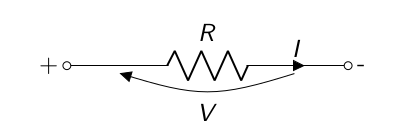
\includegraphics[width=0.5\textwidth]{Immagini/Resistenza.png}
    \caption{Rappresentazione schematica di una resistenza}
    \label{figure: resistenza}
\end{figure}
Un punto comune a due o più bipoli è detto nodo: i bipoli si possono disporre in modo tale da formare dei percorsi chiusi,
detti maglie. I concetti di nodo e maglia consentono di semplificare l'analisi di circuiti complessi per mezzo delle 
\textit{Leggi di Kirchoff}. La \textit{KVL (Kirchoff Voltage Law)} afferma che lungo una qualsiasi maglia di un circuito
la somma algebrica di tutte le tensioni è pari a zero:
\begin{equation}
    \sum_{k\,\in\,maglia}V_k\,=\,0,
    \label{equation: KVL}
\end{equation}
dove si considerano positive le tensioni concordi con il verso di percorrenza della maglia e negative le tensioni discordi.
La \textit{KCL (Kirchoff Current Law)} riguarda invece le correnti ed evidenzia come in un qualsiasi nodo di un circuito
la somma algebrica di tutte le correnti è identicamente nulla
\begin{equation}
    \sum_{k\,\in\,maglia}I_k\,=\,0,
    \label{equation: KCL}
\end{equation}
dove sono positive le $I_k$ entranti nel nodo, mentre negative quelle uscenti.
\begin{figure}[H]
    \centering
    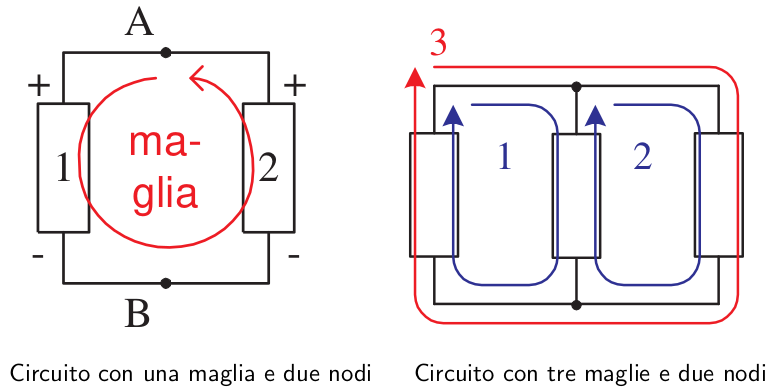
\includegraphics[width=0.9\textwidth]{Immagini/EsempioMaglie.png}
    \caption{Esempi di maglie in un circuito}
    \label{figure: KirchoffLaws}
\end{figure}
Un altro esempio di bipolo è il \textbf{condensatore}, che è un elemento circuitale costituito da due superfici metalliche 
parallele separate da un isolante. Le armature metalliche possono immagazzinare della carica, in quantità proporzionale alla
tensione applicata
\begin{equation}
    q(t)\,=\,Cv(t),
    \label{equation: capacità}
\end{equation}
dove con $C$ si indica la capacità del condensatore, misurata in farad (F).
\begin{figure}[H]
    \centering
    \includegraphics[width=0.5\textwidth]{Immagini/Capacità.png}
    \caption{Rappresentazione schematica di un condensatore}
    \label{figure: resistenza}
\end{figure}
L'ultimo esempio di bipolo a cui siamo interessati è l'\textbf{induttore}, che è costituito da un filo di materiale
conduttore percorso da corrente (solenoide).
All'interno dell'avvolgimento si ha un flusso di campo magnetico $\Phi$ che è proporzionale alla corrente che percorre il
filo
\begin{equation}
    \Phi(t)\,=\,Li(t),
    \label{equation: induttanza}
\end{equation}
dove $L$ è l'induttanza dell'induttore e si misura in henry (H).
\begin{figure}[H]
    \centering
    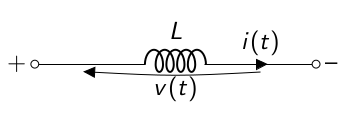
\includegraphics[width=0.5\textwidth]{Immagini/Induttanza.png}
    \caption{Rappresentazione schematica di un induttore}
    \label{figure: induttanza}
\end{figure}

\subsection{Circuito RC}

Il circuito RC è un circuito del primo ordine, ossia è caratterizzato da un'equazione differenziale del primo ordine. 
\begin{figure}[H]
    \centering
    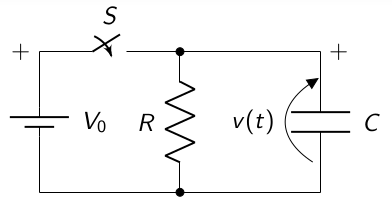
\includegraphics[width=0.65\textwidth]{Immagini/CircuitoRC.png}
    \caption{Rappresentazione schematica di un circuito RC}
    \label{figure: CircuitoRC}
\end{figure}
Gli elementi circuitali presenti sono tre:
\begin{itemize}
    \item un interruttore ideale $S$ che si comporta come un circuito aperto quando è spento e come un cortocircuito quando
    è acceso
    \item una resistenza $R$
    \item un condensatore $C$
\end{itemize}
Quando l'interruttore è acceso si assiste ad una carica del condensatore: la differenza di potenziale $v(t)$ è pari a quella
dovuta al generatore di tensione $V_0$. Mediante le semplici relazioni \eqref{equation: OhmLaw} e \eqref{equation: capacità}
introdotte in precedenza è possibile ricavare i valori di corrente nel resistore e di carica immagazzinata nel condensatore.
Supponiamo ora di aprire l'interruttore scollegando di fatto il generatore di tensione: per risolvere il circuito occorre
lavorare con le leggi di Kirchoff. In particolare notiamo che
\begin{equation}
    i_R\left(t\right)\,+\,i_C\left(t\right)\,=\,0,
    \label{equation: KCL_circuitoRC}
\end{equation}
dove gli indici si riferiscono ai due elementi circuitali presente nell'unica maglia del circuito RC una volta aperto.
La relazione \eqref{equation: KCL_circuitoRC} è un'equazione differenziale del primo ordine per la differenza di potenziale
ai capi del condensatore, poichè effettuando le opportune sostituizioni è possibile mostrare come 
\begin{equation}
    \frac{v\left(t\right)}{R}\,+\,C\frac{dv\left(t\right)}{dt}=\,0.
    \label{equation: EqDiff_circuitoRC}
\end{equation}
Notiamo che la soluzione di \eqref{equation: EqDiff_circuitoRC} sia un esponenziale reale, che imponendo la condizione iniziale
di potenziale al tempo dello spegnimento dell'interruttore pari a $V_0$ risulta essere
\begin{equation}
    v\left(t\right)\,=\,V_0\exp{\left(-\frac{t}{RC}\right)}.
    \label{equation: solEqDiff_circuitoRC}
\end{equation}


%----------------------------------------------------------------------%
%                           Seconda sezione                            %
%----------------------------------------------------------------------%
% Nella seconda sezione faccio un rapido ripasso sulla trasformata di  %
% Fourier in modo tale da introdurre come lo studio delle equazioni    %
% differenziali nel dominio delle frequenze si traduca nel trovare le  %
% soluzioni di equazioni algebriche. Fornisco un esempio di questo     %
% processo con la risoluzione del circuito RC passa basso              %
%----------------------------------------------------------------------%


\section{Dominio delle frequenze}

Lavorare nello spazio delle frequenze per risolvere i circuiti elettrici è vantaggioso, perchè si assiste ad una notevole
semplificazione dei calcoli da compiere: le equazioni differenziali presenti nel dominio del tempo che governano il comportamento
dei circuiti RLC (resistori, induttori, condensatori) diventano delle relazioni algebriche. Nel dominio delle frequenze gli
elementi circuitali che abbiamo precedentemente introdotto sono rappresentati in termini di impedenza o ammettenza, che si
comportano come resistenze in un'analisi algebrica: questo rende più immediata l'analisi dei circuiti. Nel dominio delle
frequenze è anche possibile effettuare un'analisi della risposta in frequenza, cruciale per la progettazione di filtri.

\subsection{Trasformata di Fourier}

Un segnale è periodico quando si ripete identicamente dopo un intervallo di tempo $T$, detto periodo: l'inverso del periodo
è la frequenza e viene solitamente indicata con la lettera $f$. Ogni \textbf{segnale periodico} $x(t)$ con periodo $T\,=\,1/f_0$ può+
essere espresso come \textbf{serie di Fourier}
\begin{equation}
    x\left(t\right)\,=\,\frac{1}{2}a_0\,+\,\sum_{k\,=\,1}^{\infty}\left[a_k\cos{\left(2k\pi f_0t\right)}\,+\,b_k\sin{\left(2k\pi f_0t\right)}\right],
    \label{equation: SerieFourier}
\end{equation}
dove $a_k$ e $b_k$ sono detti coefficienti di Fourier e si ottengono mediante integrazione su un periodo del segnale di partenza
che si vuole ricostruire
\begin{equation}
    a_k\,=\,\frac{2}{T}\int_{-\frac{T}{2}}^{\frac{T}{2}} x\left(t\right)\cos{\left(2k\pi f_0t\right)}dt,
    \label{equation: a_coeffFourier}
\end{equation}
\begin{equation}
    b_k\,=\,\frac{2}{T}\int_{-\frac{T}{2}}^{\frac{T}{2}} x\left(t\right)\sin{\left(2k\pi f_0t\right)}dt.
    \label{equation: b_coeffFourier}
\end{equation}
Lavorando con le \textit{formule di Eulero} per il seno ed il coseno è possibile scrivere la serie di Fourier in forma complessa:
\begin{equation}
    x\left(t\right)\,=\,\sum_{k\,=\,-\infty}^{\infty}c_k \exp{\left(j2k\pi f_0t\right)},
    \label{equation: Compl_SerieFourier}
\end{equation}
dove $c_k$ sono dei coefficienti complessi tali per cui
\begin{equation}
    c_k\,=\,c_{-k}^*\,=\,\frac{a_k\,-\,jb_k}{2}\,=\,\frac{1}{T}\int_{-\frac{T}{2}}^{\frac{T}{2}} x(t)\exp{\left(-j2k\pi f_0t\right)} dt
    \label{equation: complex_coeff}
\end{equation}
Un segnale non periodico può essere considerato come un segnale periodico caratterizzato da un periodo tendente ad infinito
(e di conseguenza una frequenza caratteristica tendente a zero): in questo caso l'analisi di Fourier prevede il passaggio
dalla sommatoria all'integrale. Si identifica con il nome \textbf{Trasformata di Fourier} di un segnale $x\left(t\right)$ la
seguente quantità:
\begin{equation}
    X\left(f\right)\,=\,\mathcal{F}\left(x\left(t\right)\right)\,=\,\int_{-\infty}^{\infty}x\left(t\right)\exp\left(-j2\pi ft\right) dt.
    \label{equation: FourierTransform}
\end{equation}
L'anti-trasformata consente di effettuare il passaggio inverso, ossia da dominio delle frequenze al dominio del tempo e si
differenzia dalla trasformata per il segno dell'esponente (che è quindi positivo nel caso di $\mathcal{F^{-1}}$) e per il
fatto che l'integrazione viene effettuata sulle frequenze.

La trasformata di Fourier consente di studiare le equazioni differenziali che risolvono i circuiti nello spazio delle frequenze, 
dove figurano come equazioni algebriche: questo è possibile poichè valgono le seguenti relazioni
\begin{equation}
    \frac{dx\left(t\right)}{dt}\,\longleftrightarrow\,j2\pi fX\left(f\right),
    \label{equation: fourierDerivata}
\end{equation}
\begin{equation}
    \int x\left(t\right)dt\,\longleftrightarrow\,\frac{1}{j2\pi f}X\left(f\right).
    \label{equation: fourierIntegrale}
\end{equation}

\subsection{Impedenza}

Passando dal dominio del tempo al dominio della frequenza per mezzo della trasformata di Fourier, notiamo che vale per tutti
e tre gli elementi circuitali una relazione lineare fra intensità di corrente e differenza di potenziale: è infatti possibile
scrivere che
\begin{equation}
    V\left(f\right)\,=\,Z\left(f\right)I\left(f\right),
    \label{equation: impedenza}
\end{equation}
dove $Z\left(f\right)$ è l'impedenza, una quantità che si misura in ohm e che per elementi circuitali in serie o in parallelo
si compone analogamente ad una resistenza.
\begin{figure}[H]
    \centering
    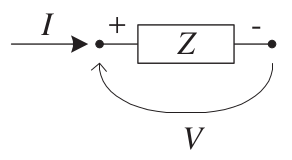
\includegraphics[width=0.35\textwidth]{Immagini/Impedenza.png}
    \caption{Rappresentazione schematica di un'impedenza}
    \label{figure: Impedenza}
\end{figure}
Nei casi dei tre bipoli presi in considerazione le impedenze sono differenti fra loro, infatti si ha che nel caso di:
\begin{equation}
    \text{un resistore} \longleftrightarrow Z\left(f\right)\,=\,R
    \label{equation: impedenzaR}
\end{equation}
\begin{equation}
    \text{un'induttanza} \longleftrightarrow Z\left(f\right)\,=\,j2\pi fL
    \label{equation: impedenzaL}
\end{equation}
\begin{equation}
    \text{un condensatore} \longleftrightarrow Z\left(f\right)\,=\,\frac{1}{j2\pi fL}
    \label{equation: impedenzaC}
\end{equation}
L'impedenza $Z$ è una grandezza complessa: la sua parte reale è la resistenza $R$, mentre la parte immaginaria prende il
nome di reattanza $X$.

\subsection{Risposta in frequenza}

La \textbf{risposta in frequenza} $H\left(f\right)$ di un circuito è definita come il rapporto fra i segnali di uscita e di
ingresso nel dominio della frequenza, ossia come
\begin{equation}
    H\left(f\right)\,=\,\frac{X_o(f)}{X_i(f)},
    \label{equation: rispostaFrequenza}
\end{equation}
dove con $X_i\left(f\right)$ e $X_o\left(f\right)$ sono indicate le trasformate di Fourier dei segnali in ingesso ed in uscita 
da un circuito. Solitamente la risposta in frequenza (che è una quantità complessa) viene espressa in termini di modulo 
$|H\left(f\right)|$ e fase $\angle H\left(f\right)$, ossia in coordinate polari nel piano complesso: i diagrammi di Nyquist 
sono la rappresentazione della traiettoria di $H\left(f\right)$ nel piano complesso.
\begin{figure}[H]
    \centering
    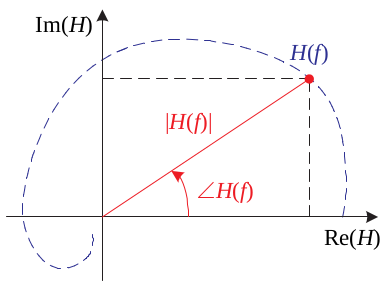
\includegraphics[width=0.35\textwidth]{Immagini/DiagrammaNyquist.png}
    \caption{Esempio di diagramma di Nyquist}
    \label{figure: Impedenza}
\end{figure}
Notiamo che se l'ingresso è unitario, l'uscita coinciderà con la risposta in frequenza: dato che $X_i\left(f\right)\,=\,1$ se
se $x_i\left(t\right)\,=\,\delta\left(t\right)$, concludiamo che $H\left(f\right)$ è la trasformata di Fourier della risposta
ad un impulso (risposta impulsiva).

\subsubsection{Diagrammi di Bode}

Per rappresentare graficamente $H\left(f\right)$ si utilizzano i \textbf{diagrammi di Bode}. Tali grafici sono di due tipi:
\begin{itemize}
    \item per le \textbf{ampiezze}, dove in ascissa si riporta la frequenza $f$ in scala logaritmica, mentre in ordinata il
          modulo del guadagno in decibel.
    \item per la \textbf{fase}, che è analogo al precedente per quanto riguarda le scisse, mentre in ordinata riporta lo 
          sfasamento.
\end{itemize}

\subsection{Circuito RC passa-basso}

Un filtro passa-basso è un sistema che permette il passaggio di frequenze al di sotto di una data soglia, detta frequenza
di taglio, bloccando le alte frequenze. Un esempio di circuito passa-basso passivo è il circuito RC presente in Figura
\ref{figure: RC_PassaBasso}, dove il segnale di output $v_{out}$ è preso fra il resistore ed il condensatore. 
\begin{figure}[H]
    \centering
    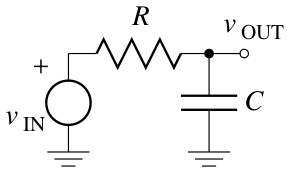
\includegraphics[width=0.35\textwidth]{Immagini/RC_PassaBasso.png}
    \caption{Rappresentazione schematica di un circuito RC passa-basso.}
    \label{figure: RC_PassaBasso}
\end{figure}
Nel dominio delle frequenze è possibile ricavare la corrente passante nella maglia come
\begin{equation}
    I\,=\,\frac{V_{in}}{Z_R\,+\,Z_C}\,=\,\frac{V_{in} \cdot j2\pi fC}{1\,+\,j2\pi fRC},
    \label{equation: corrente_RC_PB}
\end{equation}
lavorando quindi con l'impedenza totale del circuito, data in questo caso dalla somma di quelle dei due elementi circuitali.
La tensione in uscita è pari alla differenza di potenziale ai capi del condensatore, che è nuovamente possibile ottenere
ragionando in termini di impedenza
\begin{equation}
    V_{out}\,=\,Z_CI\,=\,\frac{V_{in}}{1\,+\,j2\pi fRC}.
    \label{equation: Vout_RC_PB}
\end{equation}
Abbiamo ora tutti gli ingredienti per procedere con il calcolo della risposta in frequenza
\begin{equation}
    H\left(f\right)\,=\,\frac{V_{out}}{V_{in}}\,=\,\frac{1}{1\,+\,j2\pi fRC},
    \label{equation: Risposta_RC_PB}
\end{equation}
da cui con semplici passaggi algebrici possiamo determinare i diagrammi di Bode.
\begin{figure}[H]
    \centering
    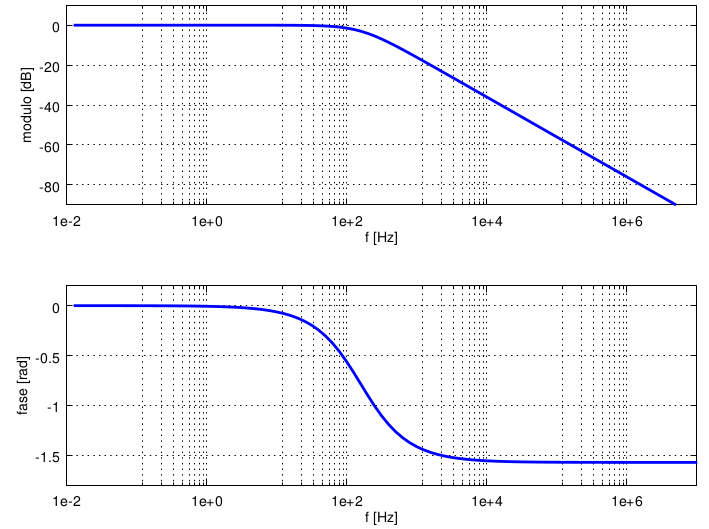
\includegraphics[width=0.75\textwidth]{Immagini/DiagrammiBodePassaBasso.png}
    \caption{Diagrammi di Bode del circuito $RC$ passa-basso.}
    \label{figure: DiagrammiBodePassaBasso}
\end{figure}

\subsection{Circuito RC passa-alto}

L'RC passa alto (vedi Figura \ref{figure: RC_PassaAlto}) è un esempio di filtro passa-alto, ossia è un circuito elettrico che
permette solo il passaggio di frequenze al di sopra di un dato valore detto frequenza di taglio.
\begin{figure}[H]
    \centering
    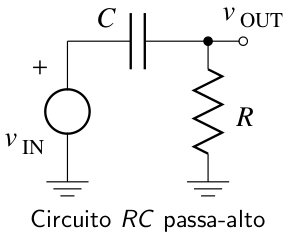
\includegraphics[width=0.35\textwidth]{Immagini/RC_PassaAlto.png}
    \caption{Rappresentazione schematica di un circuito RC passa-alto.}
    \label{figure: RC_PassaAlto}
\end{figure}
Il ragionamento che porta alla determinazione della risposta in frequenza è analogo a quello fatto nella sezione precedente.
Partendo dalla corrente I nella maglia, data anche in questo caso dalla relazione \eqref{equation: corrente_RC_PB} è possibile
ricavare il segnale in uscita come
\begin{equation}
    V_{out}\,=\,RI\,=\,\frac{V_{in} \cdot j2\pi fRC}{1\,+\,j2\pi fRC},
    \label{equation: Vout_RC_PA}
\end{equation}
con conseguente risposta in frequenza pari a
\begin{equation}
    H\left(f\right)\,=\,\frac{V_{out}}{V_{in}}\,=\,\frac{j2\pi fRC}{1\,+\,j2\pi fRC}.
    \label{equation: Risposta_RC_PA}
\end{equation}
\begin{figure}[H]
    \centering
    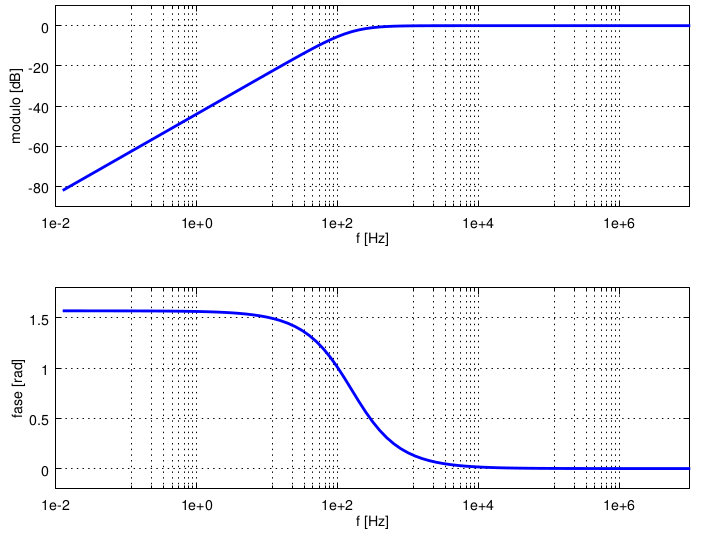
\includegraphics[width=0.75\textwidth]{Immagini/DiagrammiBodePassaAlto.png}
    \caption{Diagrammi di Bode del circuito $RC$ passa-alto.}
    \label{figure: DiagrammiBodePassaAlto}
\end{figure}

\section{L'amplificatore operazionale}

I generatori di tensione possono essere di due tipologie:
\begin{itemize}
    \item indipendenti, ossia generano grandezze elettriche indipendentemente da qualsiasi altra grandezza presente nel
    circuito.
    \item dipendenti, ossia la grandezza elettrica generata (tensione o corrente) ha un valore che è funzione di un'altra 
    grandezza elettrica presente nel circuito.
\end{itemize}
L'amplificatore operazionale (detto anche \textbf{OpAmp}) è un generatore di tensione controllato in tensione che 
amplifica la differenza di tensione tra i due segnali di ingresso $V^+$ e $V^-$: con '+' viene indicato l'ingresso
\textit{'non invertente'}, mentre con '-' l'ingresso \textit{'invertente'}. 
\begin{figure}[H]
    \centering
    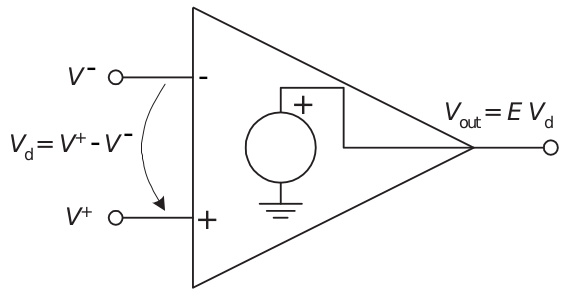
\includegraphics[width=0.45\textwidth]{Immagini/OpAmp.png}
    \caption{Rappresentazione schematica dell'amplificatore operazionale.}
    \label{figure: OpAmp}
\end{figure}
Il guadagno di tensione dell'OpAmp è infinito, ossia
\begin{equation}
    V_{out}\,=\,EV_d\,=\,E\left(V^+\,-\,V^-\right)\qquad \text{con} \qquad E \rightarrow \infty.
    \label{equation: Out_OpAmp}
\end{equation}
Solitamente l'amplificatore viene utilizzato in \textit{configurazione retroazionata}: il segnale in uscita è riportato all'
ingresso mediante una rete di retroazione costituita da elementi passivi come per esempio resistori. Sono possibili due tipologie
di retroazione:
\begin{itemize}
    \item positiva, con segnale d'uscita riportato all'ingresso non invertente.
    \item negativa, con segnale d'uscita riportato all'ingresso invertente.
\end{itemize}
I circuiti retroazionati hanno un comportamento simile a quello di una pallina appoggiata ad una superficie curva: possono
essere stabili oppure instabili. 

\subsection{Amplificatore invertente}

Il circuito che stiamo prendendo in considerazione presenta un solo amplificatore operazionale ideale: la rete di retroazione
riporta il segnale all'ingresso invertente (ossia identificato con  il segno meno sullo schema dell' OpAmp).
\begin{figure}[H]
    \centering
    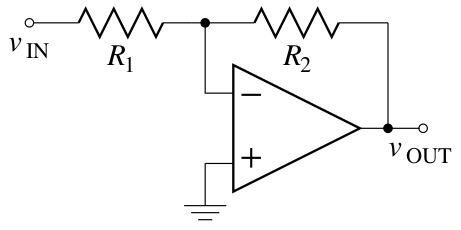
\includegraphics[width=0.45\textwidth]{Immagini/AmplificatoreInvertente.png}
    \caption{Rappresentazione schematica dell'amplificatore invertente.}
    \label{figure: OpAmp}
\end{figure}
Il circuito preso in analisi può essere descritto mediante il seguente sistema di equazioni:
\begin{equation}
    \begin{cases}
        V_{in}\,-\,V^{-}\,=\,R_1I_1 \\
        V^-\,-\,V_{out}\,=\,R_2I_2  \\
        I_1\,=\,I_2 \\
        V_{out}\,=\,E\left(V^+\,-\,V^-\right)\,=\,-EV^-
    \end{cases}
    \label{equation: sistema_AmpInv}
\end{equation}
Dato che il guadagno $E$ dell'amplificatore operazionale ideale è infinito, l'ultima equazione è risolvibile solamente se
assume la forma indeterminata $\infty \cdot 0$: in tal caso il prodotto può assumere un valore finito. Sfruttando ora 
l'uguaglianza fra le due correnti è possibile verificare come
\begin{equation}
    V_{out}\,=\,-\frac{R_2}{R_1}V_{in},
    \label{equation: Vout_AmpInv}
\end{equation}
evidenziando come in questo circuito il guadagno dipenda solamente dal rapporto fra le due resistenze: la presenza del meno
giustifica la qualifica di \textit{invertente}.

\subsection{Amplificatore non invertente}

Un amplificatore che produce in uscita un segnale amplificato, avente una fase simile a quella dell'ingresso applicato, è 
detto amplificatore non invertente. 
\begin{figure}[H]
    \centering
    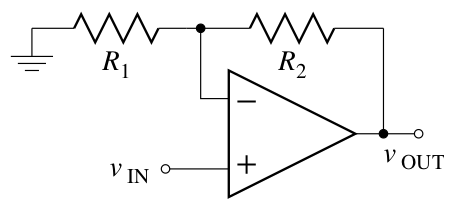
\includegraphics[width=0.45\textwidth]{Immagini/AmplificatoreNonInvertente.png}
    \caption{Rappresentazione schematica dell'amplificatore non invertente.}
    \label{figure: OpNonAmp}
\end{figure}
La rete di retroazione è identica al caso precedente: dato che la retroazione è negativa
possiamo nuovamente applicare il principio di terra virtuale, ossia:
\begin{equation}
    \begin{cases}
        V^-\,=\,V^+\,=\,V_{in}  \\
        I^-\,=\,I^+\,=\,0
    \end{cases}
    \label{equation: TerraVirtuale}
\end{equation}
Andando nuovamente ad uguagliare le correnti passanti nelle due resistenze ricaviamo che
\begin{equation}
    -\frac{V_{in}}{R_1}\,=\,\frac{V_{in}\,-\,V_{out}}{R_2},
    \label{equation: equal_current}
\end{equation}
da cui banalmente segue che
\begin{equation}
    V_{out}\,=\,\left(1\,+\,\frac{R_2}{R_1}\right)
    \label{equation: Vout_signal}
\end{equation}


\newpage

\end{document}


